\chapter{Results}
\section{Laser Current Driver}
\subsection{Zener Diode Selection}
Chinese/Ebay Zeners. Welded legs. Photots. Decap one of those.

\subsection{Building a Test Setup for Zener Diodes}
In order to test a large amount of Zener diodes, and considering the duration of the burn-in process, which can take anything between \qtyrange{100}{1000}{\hour}, it is neccesary to have an automated setup. This consists of a digital multimeter (DMM) a scanner and test board, that holds the zener diodes and provides the neccesary infrastructure for the diodes.

The type of DMM used, plays an important role. The expected amplitude of the popcorn noise is around \qty{4}{\micro\volt}. To measure the \qty{7}{\volt} of the zener diode, the corresponding voltage range of a typical DMM would be either \qty{10}{\volt} or \qty{20}{\volt}. This means, that either a very low noise \num{7.5} or an \num{8.5} digit multimeter is required to record the popcorn noise. Fortunately, this class of multimeters features a superior voltage reference, because the LM399 is not suitable for \num{8.5} digits as it is too noisy. The only Zener diodes good enough are the Analog Devices LTZ1000 \cite{}, the Motorolla SZA263 (out of production) and the Linear Technology (LT) LTFLU-1 (proprietary design by Fluke and LT).  While Keysight uses the LTZ0100, Fluke either uses the SZA263 (in older devices) or the LTFLU-1 and Keithley uses both devices, the LTZ1000 in their \device{Model 2002} and the LTFLU-1 in the newer \device{DMM7510}.

In comparison to the LM399, those Zener diodes do not suffer from the popcorn noise issue. This means, that there are no additional measures required to make sure the popcorn noise is caused by the device under test (DUT) and not the DMM.

To conclude, we need a high performance DMM, a scanner, and a test fixture. The choices will detailed in the following sections.

\subsection{Choosing a DMM for Testing Zener Diodes}
The market for high-end \num{8.5} digit DMMs is limited and therefore every device on the market caters for a certain niche. In table \ref{tab:list_of_dmms} a list of popular \num{8.5} DMMs can be found. Several models are included in the table, althought they are discontinued. The reason is, that these DMMs can still be acquired on the second-hand market.

\begin{table}[h]
    \centering
    \begin{tabular}{ |l|l|l| }
        \hline
        Manufacturer & Model & Remarks \\
        \hline
        Advantest & \device{R6581} & Discontinued. Scanner cards available. \\
        Datron/Wavetek & \device{1812} & Discontinued. Bought by Fluke. \\
        Fluke & \device{8508A} & Discontinued. \qty{20}{\volt} range. \\
        Fluke & \device{8588A} & In production. \\
        Keithley/Tektronix & \device{2002} & In production. Scanner card available. \qty{20}{\volt} range. \\
        Keysight & \device{3458A} & In Production. \\
        Solartron & \device{7081} & Discontinued. Slow. \\
        Transmille & \device{8104} & In Production. External scanner available. Slow. \\
        \hline
    \end{tabular}
    \caption{A non-exhaustive list of \num{8.5} digit multimeters.}
    \label{tab:list_of_dmms}
\end{table}

While the author has not tested every multimeter in table \ref{tab:list_of_dmms}, given a scanner solution, each of those would suffice to test the Zener diodes. The \device{Solartron 7081} (also sold as \device{Guildline 9578}) is a less optimal choice, because a conversion takes \qty{52}{\s} for \num{8.5} digits, but it would still be workable. The discontinued \device{Fluke 8508A} and the \device{Wavetek 1812} multimeter are very similar as Fluke bought Wavetek in 2000 and as a result, the \device{Fluke 8508A} is more an update to the \device{Wavetek 1812} than a new device. Unfortunately, it is very rare to see one the Fluke device on the second hand market, while the \device{1812} can be found with a bit of patience.

The other multimeters still in production while all similar in price, their nice is different. The \device{Fluke 8588A} excels at stability and features a moder user interface, whereas the \device{Keysight 3458A} is unbeaten in linearity and noise. A detailed comparison of those two meters can be found in the work of \citeauthor*{article_fluke_8588A_noise} \cite{article_fluke_8588A_noise}. The \device{Keithley Model 2002} focuses on its scanning capability and the \device{Transmille 8104} does have electrometer functions. Unfortunately, the \device{8104} is also fairly slow at \num{8.5} digit with conversions taking \qty{4}{\s} \cite{datasheet_transmille8104}.

\subsection{A Scanner System for Testing Zener Diodes}
As discussed before the diodes need to be tested for \qty{1000}{\hour} and it would not be feasible to test them individually. So a minimum of 10 diodes should be tested at the same time. To keep the system compact the test setup must use some kind of scanner to multiplex a single multimeter input. Several options where considered, but a recent trend to event more compact device has led major manufacturers to include a multimeter itself in the scanner mainframe creating so called data aquistion units. For example Keithley replaced the small desktop switch mainframe \device{Model 7001} with the \device{DAQ6510} and Keysight is offering the \device{DAQ973A}, a scanning \num{6.5} digit DMM, that accepts extension cards. For this project the integrated \num{6.5} digit multimeter does not add value as discussed above and only increases the cost.

The simplest option is to go with a multimeter that already included a scanner option or if an external scanner is required, it is recommended to buy a used \device{Keithley 7001}. The author has tested both options and the simplicity of only having a single device to connect and program makes the integrated scanner card of the \device{Model 2002} very attractive.

Finally the type type of scanner card needs to be discussed.



In this work the Keithley (now Tektronix) \device{Model 2002} was chosen for three reasons. It is a very compact system requiring only a half-sized 2U rack in comparison to the other DMMs, that are typically full-sized 2U rack devices. The other two advantages are the integrated scanner card slot, that allows to to fit a 10 channel scanner card and finally the \qty{20}{\volt} range. The latter is interesting for testing the final voltage reference boards, as these have a \qty{15}{\volt} output, which is too much for the \qty{10}{\volt} range of most DMMs, so that testing the voltage reference PCBs one would have to switch to the \qty{100}{\volt} range and forgo an extra digit of resolution and add more noise.



The test setup consists of a mounting pcb, that holds up to 20 Zener diode. It provides power regulation and a minimal circuit required to support each diode. This circuit is given here:

\begin{figure}[ht]
    \centering
    \scalebox{0.7}{%
    \import{figures/}{zener_burnin.tex}
    } % scalebox
    \caption{Circuit used for burning in the Zener diodes}
\end{figure}

The compensation network is required when using the ADR1399, because of its very low dynamic impedance as recommended in the datasheet \cite{datasheet_ADR1399}. It is not strictly required for the LM399, but fitted nonetheless, because there are no downsides to it. This makes the board compatible with both types of references. Each Zener output is protected using an output buffer, which provides isolation and short circuit protection. Finally there is a common mode filter at the output to supress high frequency noise via gound loops.

The two key metrics of concern, that need to measured are popcorn noise and drift.

digital multimeter and a scanner card


\begin{figure}[ht]
    \centering
    \import{figures/}{DIN_41612.tex}
    \caption{The extension connector used in several Keithley multimeters}
\end{figure}

\begin{tabular}{llllll}
    \toprule
    Pin    & Function    & Cable Colour    & Pin    & Function    &  Cable Colour\\
    \midrule
    a1, b1    & \SIrange[explicit-sign=+]{6}{20}{\volt}    & brown    & \num{6}    & GND    & green/white\\
    a2, b2    & PD cathode (optional)    & red    & \num{7}    & LD Cathode    & blue/white\\
    a3, b3    & LD case (GND)    & red/white    & \num{8}    & LD Anode    & blue\\
    a4    & PD anode (GND)    & red/white    & \num{9}    & LD current monitor    & green\\
    a5    & \SIrange{-6}{-20}{\volt}    & brown/white\\
    \bottomrule
\end{tabular}

\begin{figure}[h]
    \centering
    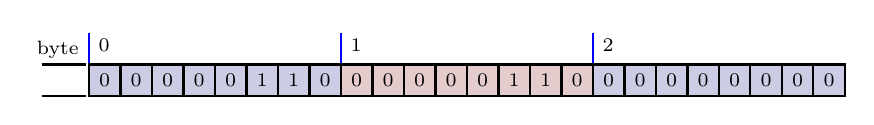
\begin{tikzpicture}[scale=0.4, text height=1.25ex, text depth=.25ex,
        bit/.style = {
            rectangle,
            thick,
            draw=black,
            inner sep=0pt,
            outer sep=0pt,
            above right,
        },
        framing/.style={
            fill=blue!50!black!20,
            minimum height = 4mm,
            minimum width = 4mm,
            bit,
        },
        command/.style = {
            fill=red!50!black!20,
            minimum height=4mm,
            minimum width=4mm,
            bit
        },
        payload/.style = {
            fill=green!50!black!20,
            minimum height=4mm,
            minimum width=4mm,
            bit
        },]
        \foreach \x in {0,...,2} {
            \node[above right] at (\x*8,1) {\scriptsize \x};
            \draw[thick, blue] (\x*8,1) -- (\x*8,2);
        }

        \node [thick, left] () at (0,1.5) {\scriptsize byte};
        \draw [thick] (-1.5, 1) -- (-0.1,1);
        \draw [thick] (-1.5, 0) -- (-0.1,0);
        % Framing start
        \begin{scope}[]
            \node[framing] at (0,0) {\scriptsize 0};
            \node[framing] at (1,0) {\scriptsize 0};
            \node[framing] at (2,0) {\scriptsize 0};
            \node[framing] at (3,0) {\scriptsize 0};
            \node[framing] at (4,0) {\scriptsize 0};
            \node[framing] at (5,0) {\scriptsize 1};
            \node[framing] at (6,0) {\scriptsize 1};
            \node[framing] at (7,0) {\scriptsize 0};
        \end{scope}

        % Command Byte
        \begin{scope}[xshift=8cm]
            \node[command] at (0,0) {\scriptsize 0};
            \node[command] at (1,0) {\scriptsize 0};
            \node[command] at (2,0) {\scriptsize 0};
            \node[command] at (3,0) {\scriptsize 0};
            \node[command] at (4,0) {\scriptsize 0};
            \node[command] at (5,0) {\scriptsize 1};
            \node[command] at (6,0) {\scriptsize 1};
            \node[command] at (7,0) {\scriptsize 0};
        \end{scope}
        % Framing end
        \begin{scope}[xshift=16cm]
            \node[framing] at (0,0) {\scriptsize 0};
            \node[framing] at (1,0) {\scriptsize 0};
            \node[framing] at (2,0) {\scriptsize 0};
            \node[framing] at (3,0) {\scriptsize 0};
            \node[framing] at (4,0) {\scriptsize 0};
            \node[framing] at (5,0) {\scriptsize 0};
            \node[framing] at (6,0) {\scriptsize 0};
            \node[framing] at (7,0) {\scriptsize 0};
        \end{scope}
    \end{tikzpicture}
\end{figure}

\subsection{Current Sources}
Discuss Op amp choice (AD797)

\subsection{Temperature Coeeficient}
Discuss each section (Reference, DAC, Buffer/Divider, Filter, CC)
\subsubsection{Voltage Reference}
\subsubsection{DAC}
\subsubsection{Divider}
\subsubsection{Filter}
Choice of components. Leakage current, size of resistor (input bias current of AD797), size of capacitor
